% Área sob a curva: soma de Riemann
% Feito para o ÉguaTeX (eguatex.com.br). Uso livre (CC0 1.0).
%
% Compile e pronto: sai só a figura, em PDF.
% Para pôr no seu trabalho, use o PDF com \includegraphics ou copie
% o bloco tikzpicture para dentro de uma figure.
%
% A altura de cada retângulo é f no ponto escolhido do subintervalo:
% 0 usa a ponta esquerda, 0.5 o ponto médio e 1 a ponta direita.
\documentclass[tikz,border=4pt]{standalone}
\usepackage[T1]{fontenc}
\usepackage{lmodern}
\usepackage{amsmath}

\colorlet{corRet}{orange!60!white}
\colorlet{corCurva}{blue!70!black}

\begin{document}
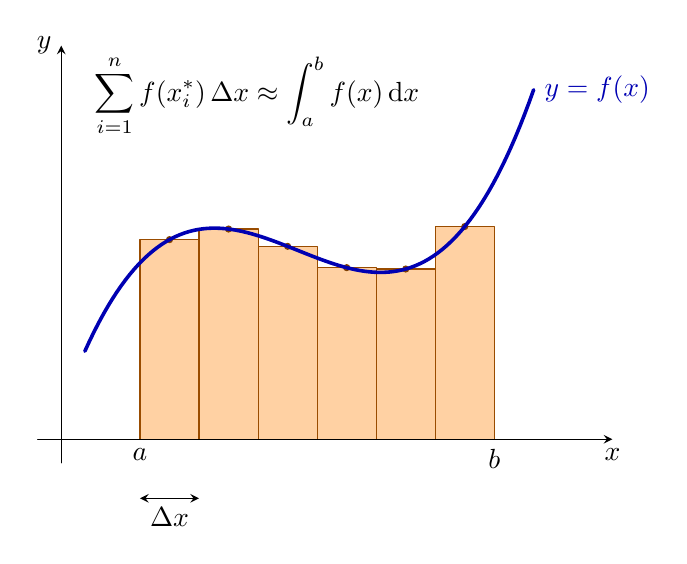
\begin{tikzpicture}[line cap=round, line join=round, >=stealth,
  % Mude a função aqui. Use valores positivos no intervalo do desenho.
  declare function={f(\x) = 0.12*(\x-3)^3 - 0.4*(\x-3) + 2.4;}]

% Mude estes números e o desenho e os rótulos acompanham.
\def\a{1}       % começo do intervalo
\def\b{5.5}     % fim do intervalo
\def\n{6}       % número de retângulos
\def\ponto{0.5} % ponto de cada subintervalo: 0, 0.5 ou 1
\def\xmax{7}    % até onde vai o eixo x
\def\ymax{5}    % até onde vai o eixo y
\def\xfim{6}    % até onde a curva vai

\pgfmathsetmacro{\dx}{(\b-\a)/\n}

% retângulos
\foreach \i in {1,...,\n} {
  \pgfmathsetmacro{\xe}{\a+(\i-1)*\dx}
  \pgfmathsetmacro{\xd}{\xe+\dx}
  \pgfmathsetmacro{\h}{f(\xe+\ponto*\dx)}
  \filldraw[fill=corRet, fill opacity=0.6, draw=orange!60!black] (\xe,0) rectangle (\xd,\h);
  \fill[orange!50!black] ({\xe+\ponto*\dx},\h) circle[radius=1.3pt];
}

% eixos
\draw[->] (-0.3,0) -- (\xmax,0) node[below] {$x$};
\draw[->] (0,-0.3) -- (0,\ymax) node[left] {$y$};
\node[below] at (\a,0) {$a$};
\node[below] at (\b,0) {$b$};
\draw[<->] (\a,-0.75) -- ({\a+\dx},-0.75) node[midway, below] {$\Delta x$};

% curva
\draw[corCurva, line width=1.3pt] plot[domain=0.3:\xfim, samples=100] (\x,{f(\x)})
  node[right] {$y=f(x)$};

% fórmula
\node[anchor=north west] at (0.3,\ymax) {$\displaystyle\sum_{i=1}^{n} f(x_i^{*})\,\Delta x \approx \int_a^b f(x)\,\mathrm{d}x$};
\end{tikzpicture}
\end{document}
